\section{Условия проведения эксперимента}

Для более объективного изучения процесса взаимодействия дискового инструмента с ПСЛО предлагается контролировать три составляющие силы резания: горизонтальную, боковую и вертикальную. Контроль этих составляющих непосредственно на рабочем органе мало эффективен, так как: требует больших трудозатрат и дорогостоящего оборудования (датчики силы, оснастка для их монтажа); невозможно изолировать влияние температуры окружающей среды, влажности, теплозапаса дорожного полотна и других факторов друг на друга; постоянно меняются физико-механические свойства ПСЛО (прочность, плотность, наличие абразивного материала). Поэтому, опираясь на результаты работ по резанию мерзлых грунтов различными инструментами \cite{JelukevichGrunt, BaronTang, BaronShar, Zelenin}, целесообразно исследовать процесс взаимодействия полноразмерного дискового режущего инструмента (см. рисунок \ref{fig:DRI}) с различным радиусом закругления рабочей кромки с разрушаемым массивом путем стендовых испытаний в лабораторных условиях.
\begin{figure}[ht]
	\centering
	\includegraphics[width=0.55\textwidth]{DRI_final}

	$R$ "--- радиус закругления рабочей кромки; $t$ "--- шаг резания; $D$ "--- диаметр дискового резца; $\delta$ "--- угол заострения; $h$ "--- глубина резания; $\gamma$ "--- задний угол. 
	\caption{Схема взаимодействия дискового режущего инструмента с разрушаемым массивом} 
	\label{fig:DRI}  
\end{figure}

При проведении экспериментальных исследований использовались дисковые резцы с различным радиусом закругления рабочей кромки $ R=[0,5; 1,5; 2,5; 3,5; 4,5] $ мм. Данный диапазон значений обусловлен результатами исследованиями изнашивания режущей кромки проведенными в работе \cite{BaronTang}. Скорость резания: $0,51\ \slantfrac{\text{м}}{\text{c}}$ ($1,84\ \slantfrac{\text{км}}{\text{ч}}$). Температура окружающего воздуха: $-2{}^\circ C\div-7{}^\circ C$. Остальные параметры дискового режущего инструмента приняты следующими: диаметр:  $D=200$ мм.; угол заострения: $\delta=30^\circ$; глубина резания: $h=60$ мм.; шаг резания: $t=[10; 20; 30; 40; 50]$ мм.; задний угол: $\gamma=3^\circ\div5^\circ$;  материал: термообработанная сталь 40ХН (HRC 52~--~54) \cite{Feshenko2017spravochik}.
% \begin{itemize}
% 	\item диаметр:  $D=200$ мм.;
% 	\item угол заострения: $\delta=30^\circ$;
% 	\item глубина резания: $h=60$ мм.;
% 	\item шаг резания: $t=[10; 20; 30; 40; 50]$ мм.;
% 	\item задний угол: $\gamma=3^\circ\div5^\circ$;
% 	\item температура окружающего воздуха: $-2{}^\circ C\div-7{}^\circ C$;
% 	\item скорость резания: $0,51\ \slantfrac{\text{м}}{\text{c}}$ ($1,84\ \slantfrac{\text{км}}{\text{ч}}$).
% \end{itemize}
Для проведения эксперимента использовался механизированный лабораторный стенд описанный в работе \cite{Sram2013Modernizaciya} конструкция которого защищена патентом на изобретение №~2429459 \cite{ExpStend}. Для фиксирования и записи информации применен измерительный комплекс описанный в статье \cite{IKI2016:my}.

\section{Тензометрический измерительный элемент}

Тензометрическая балка представляет собой тонкостенную цилиндр (рисунок \ref{fig:Zveno}) с прямоугольным основанием, служащим креплением к лабораторному стенду.% 
%
% \begin{wrapfigure}{l}{0.5\textwidth}
%   \vspace{-25pt}
%   \begin{center}
%     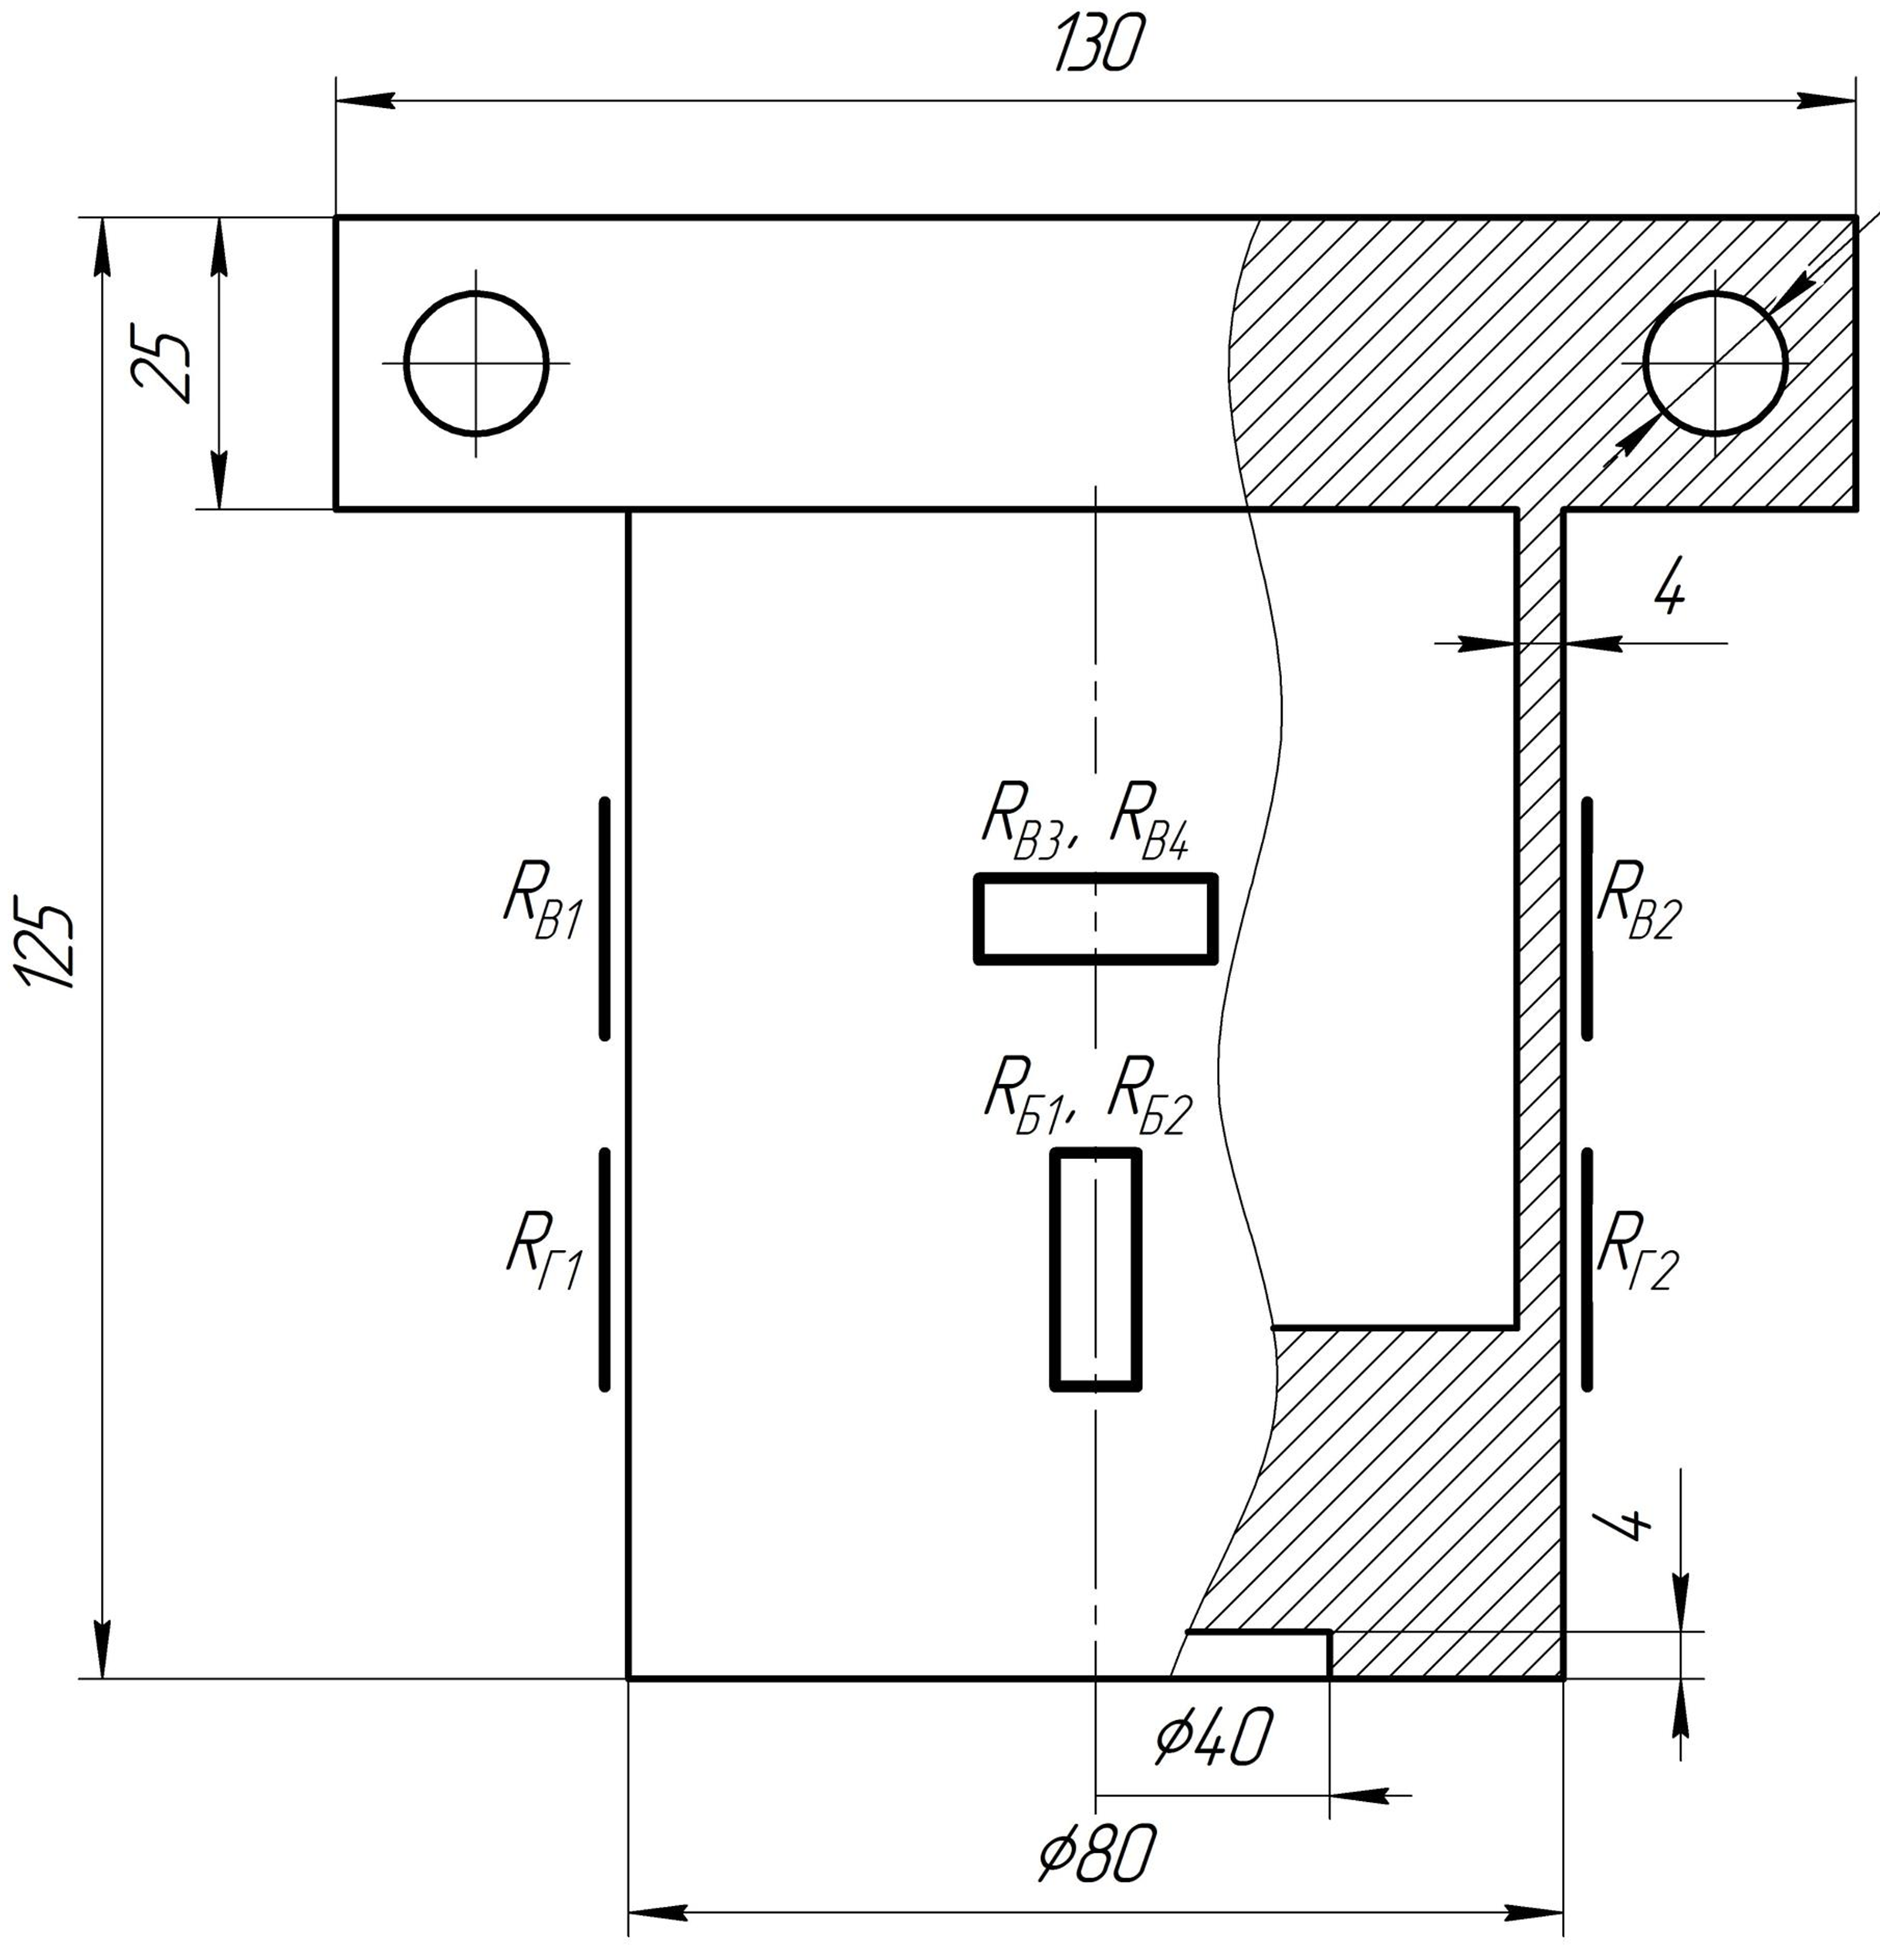
\includegraphics[width=0.5\textwidth]{ZvenoOnli}
%   \end{center}
%   \vspace{-15pt}
%   \caption{Схема наклейки тензорезисторов}
%   \label{fig:Zveno}
%   \vspace{-16pt}
% \end{wrapfigure}
\begin{figure}[!h]
	\centering
	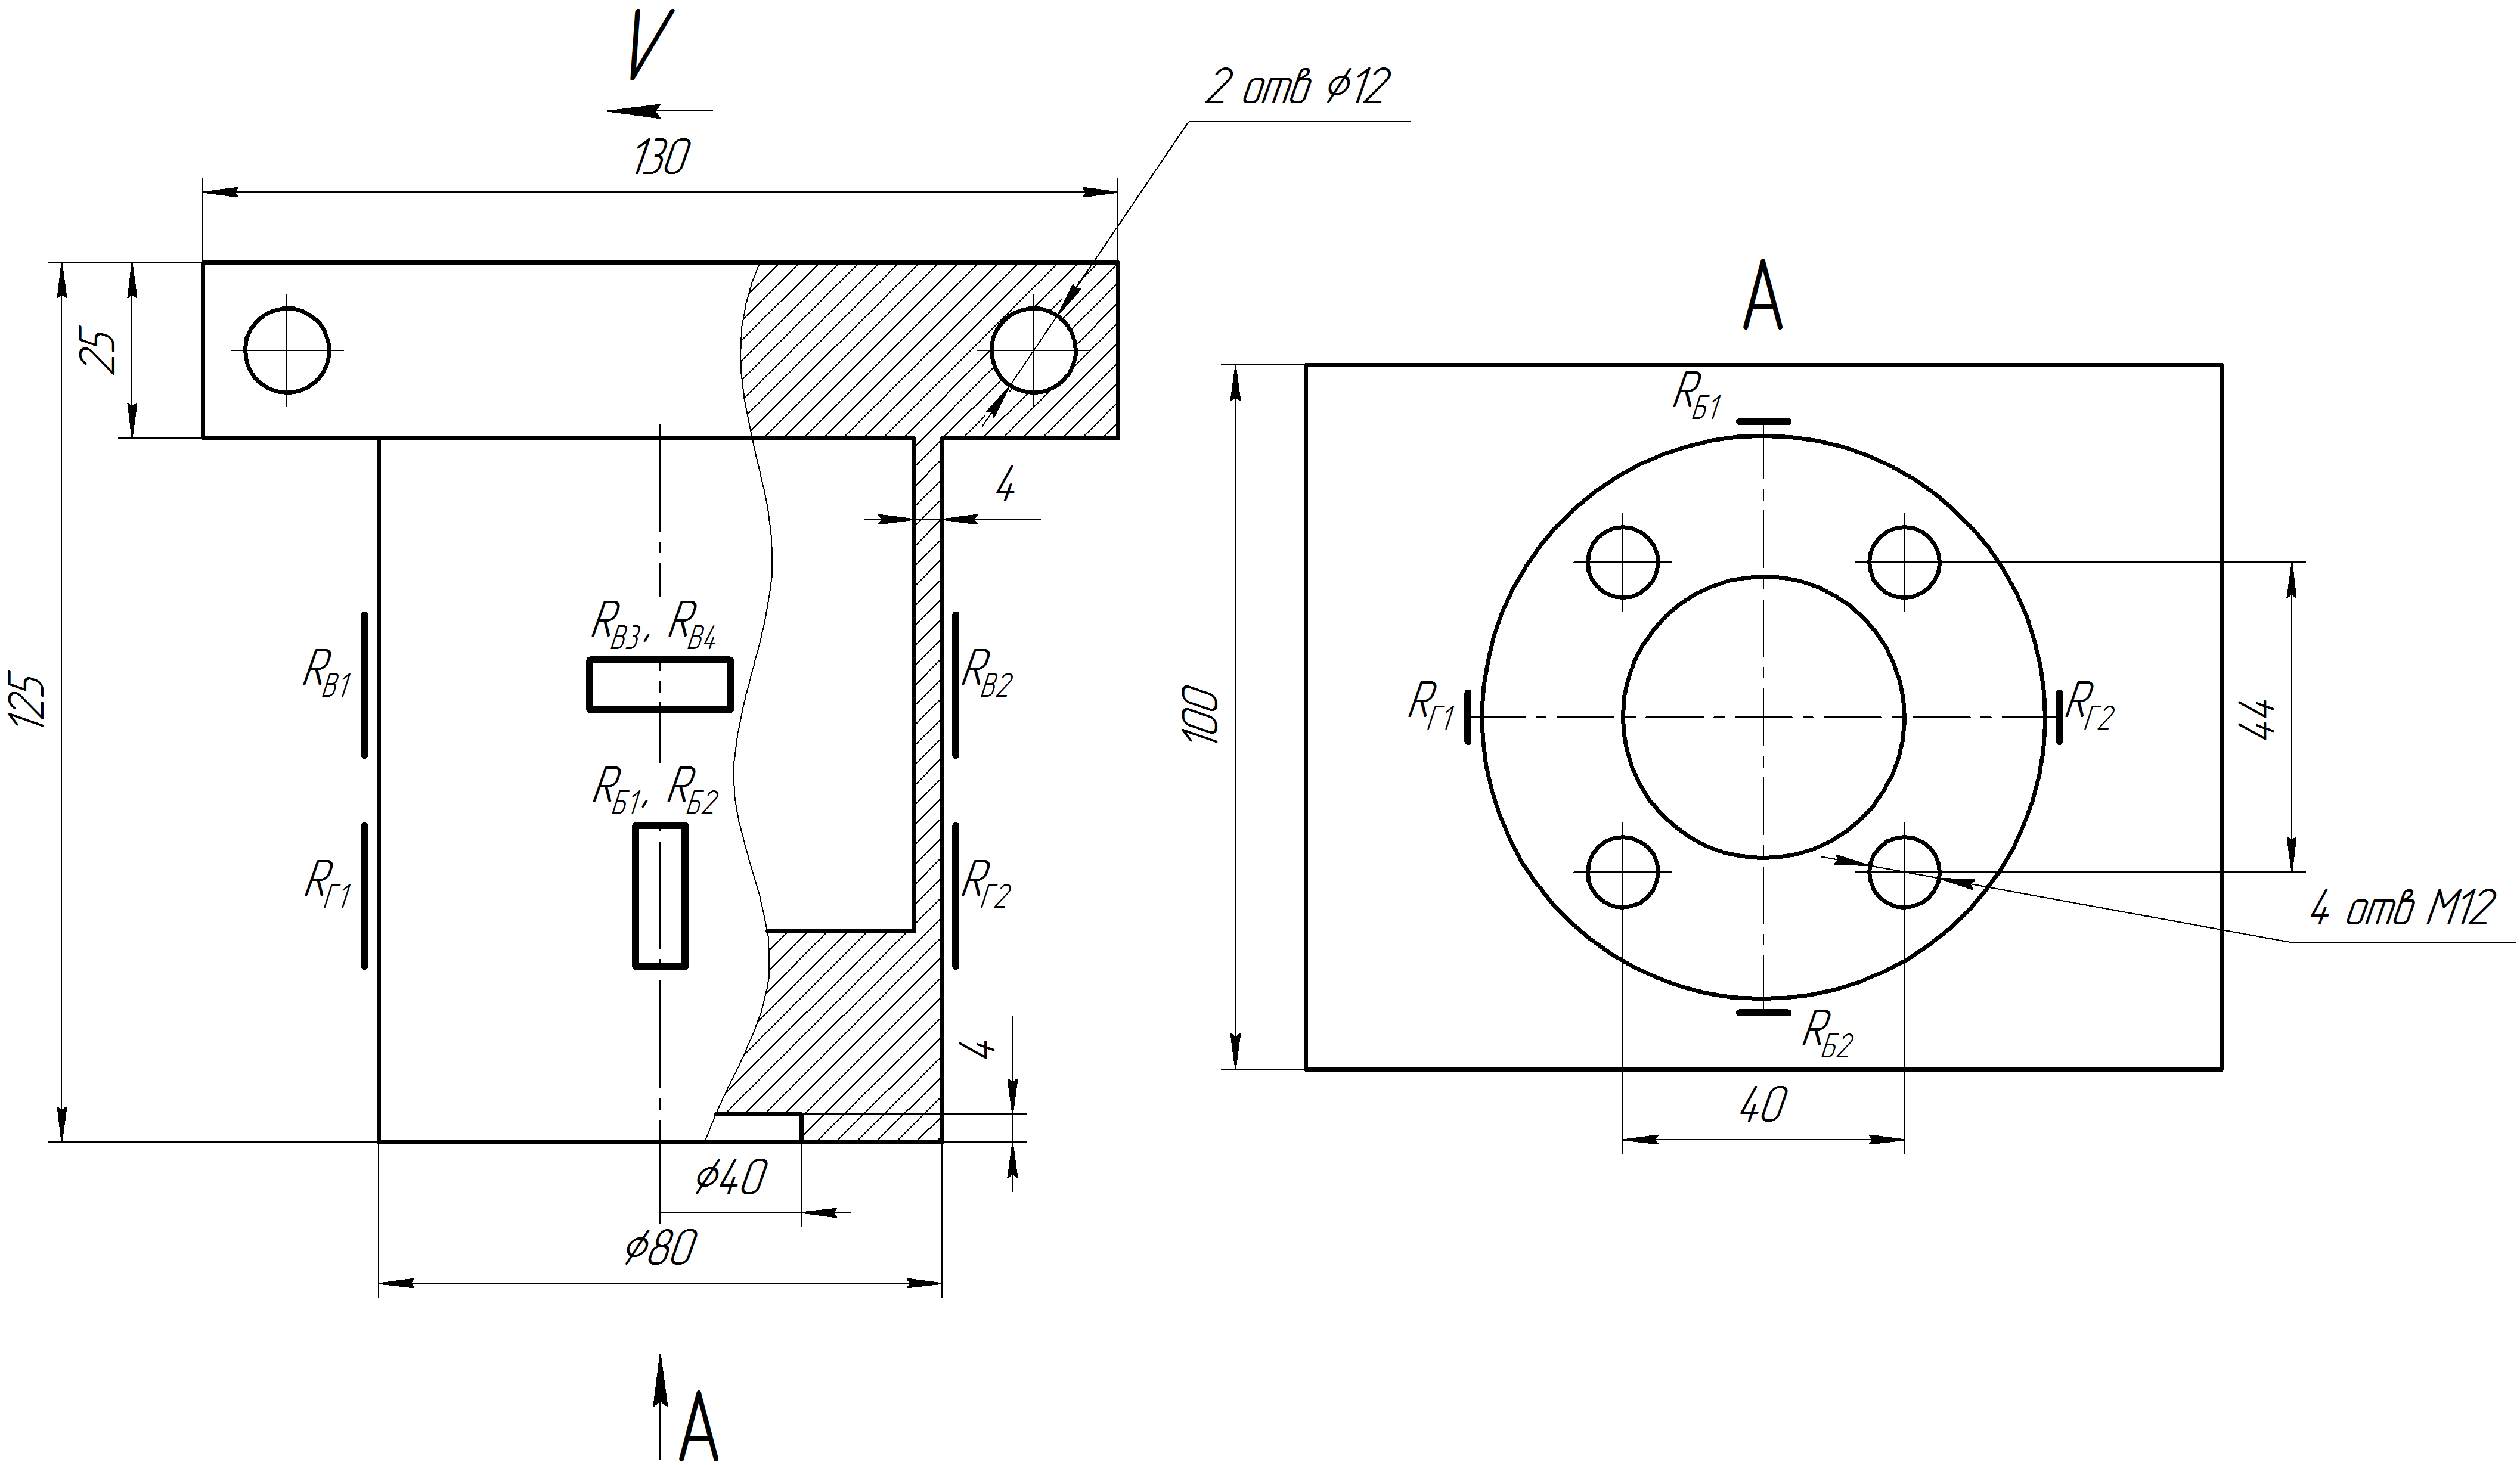
\includegraphics[width=1\textwidth]{ZvenoDWG}
	%
	%А "--- схема наклейки тензорезисторов; Б "--- общий вид тензометрического звена;
	%1 "--- тензометрическая головка; 2 "--- крепёж дискового режущего инструмента
	\caption{Чертеж тензометрического измерительного элемента} 
	\label{fig:Zveno}  
\end{figure}
Изделие выполнено из стали марки \textit{55С2} \cite{Feshenko2017spravochik}. При приложении усилий к такой балке происходит её упругая деформация, на которую реагируют наклеенные на неё тензорезистивные элементы (2ФКПА 20~200 ГВ) путем изменения своего сопротивления. На рисунке \ref{fig:Zveno} приведена схема наклейки чувствительных элементов.

Для измерения горизонтальной составляющей приложенного усилия используется полумостовая схема включения, с избирательной чувствительностью, тензорезистор $R_\textit{Г1}$ включён в первое плечо измерительного моста, а $R_\textit{Г2}$ – в четвёртое. Такая схема позволяет обеспечить избирательную чувствительность тензометрического моста к деформации изгиба, возникающей в следствии действия горизонтальной составляющей приложенного усилия, и не чувствительна к деформации растяжения-сжатия, возникающей в следствии действия вертикальной составляющей. Для боковой составляющей используется схема включения тензорезисторов аналогичная приведённой выше. Тензорезистор $R_\textit{Б1}$ включён в первое плечо измерительного моста, а $R_\textit{Б2}$ – в четвёртое. Для измерения вертикальной составляющей, диаметрально расположенные тензорезисторы $R_\textit{В1}$ и $R_\textit{В2}$ необходимо включить в одно плечо полумоста. Во второе плечо включаются компенсационные тензорезисторы $R_\textit{В3}$ и $R_\textit{В4}$, обеспечивающие также термокомпенсацию. Все схемы включения обеспечивают термокомпенсацию и компенсацию сопротивления соединительных проводов.

\section{Тарирование тензометрического звена}

Для тарирования тензометрического звена, описанного выше, применялся стенд, конструкция которого защищена патентом на изобретение №~2500983 \cite{CalibrationStend}, позволяющий закреплять звено в различных пространственных положения и соответственно создавать требуемый вектор нагрузки. Тарирование производилось с помощью: одного измерительного прибора "--- динамометра растяжения ДПУ-5-2~5033 второго класса точности; талрепа и вспомогательной оснастки для крепежа тензометрического звена.

Нагрузка звена осуществлялась ступенчато, с шагом 500~Н, до предельного значения в 2~500~Н. Разгрузка производилась с тем же шагом до нулевого значения. На рисунке~\ref{fig:CalibrationRawHor} приведена диаграмма переходных процессов возникающих во время тарирования. Из неё явно видно, что исключено взаимное влияние составляющих друг на друга.
\begin{figure} [ht]
	\centering
	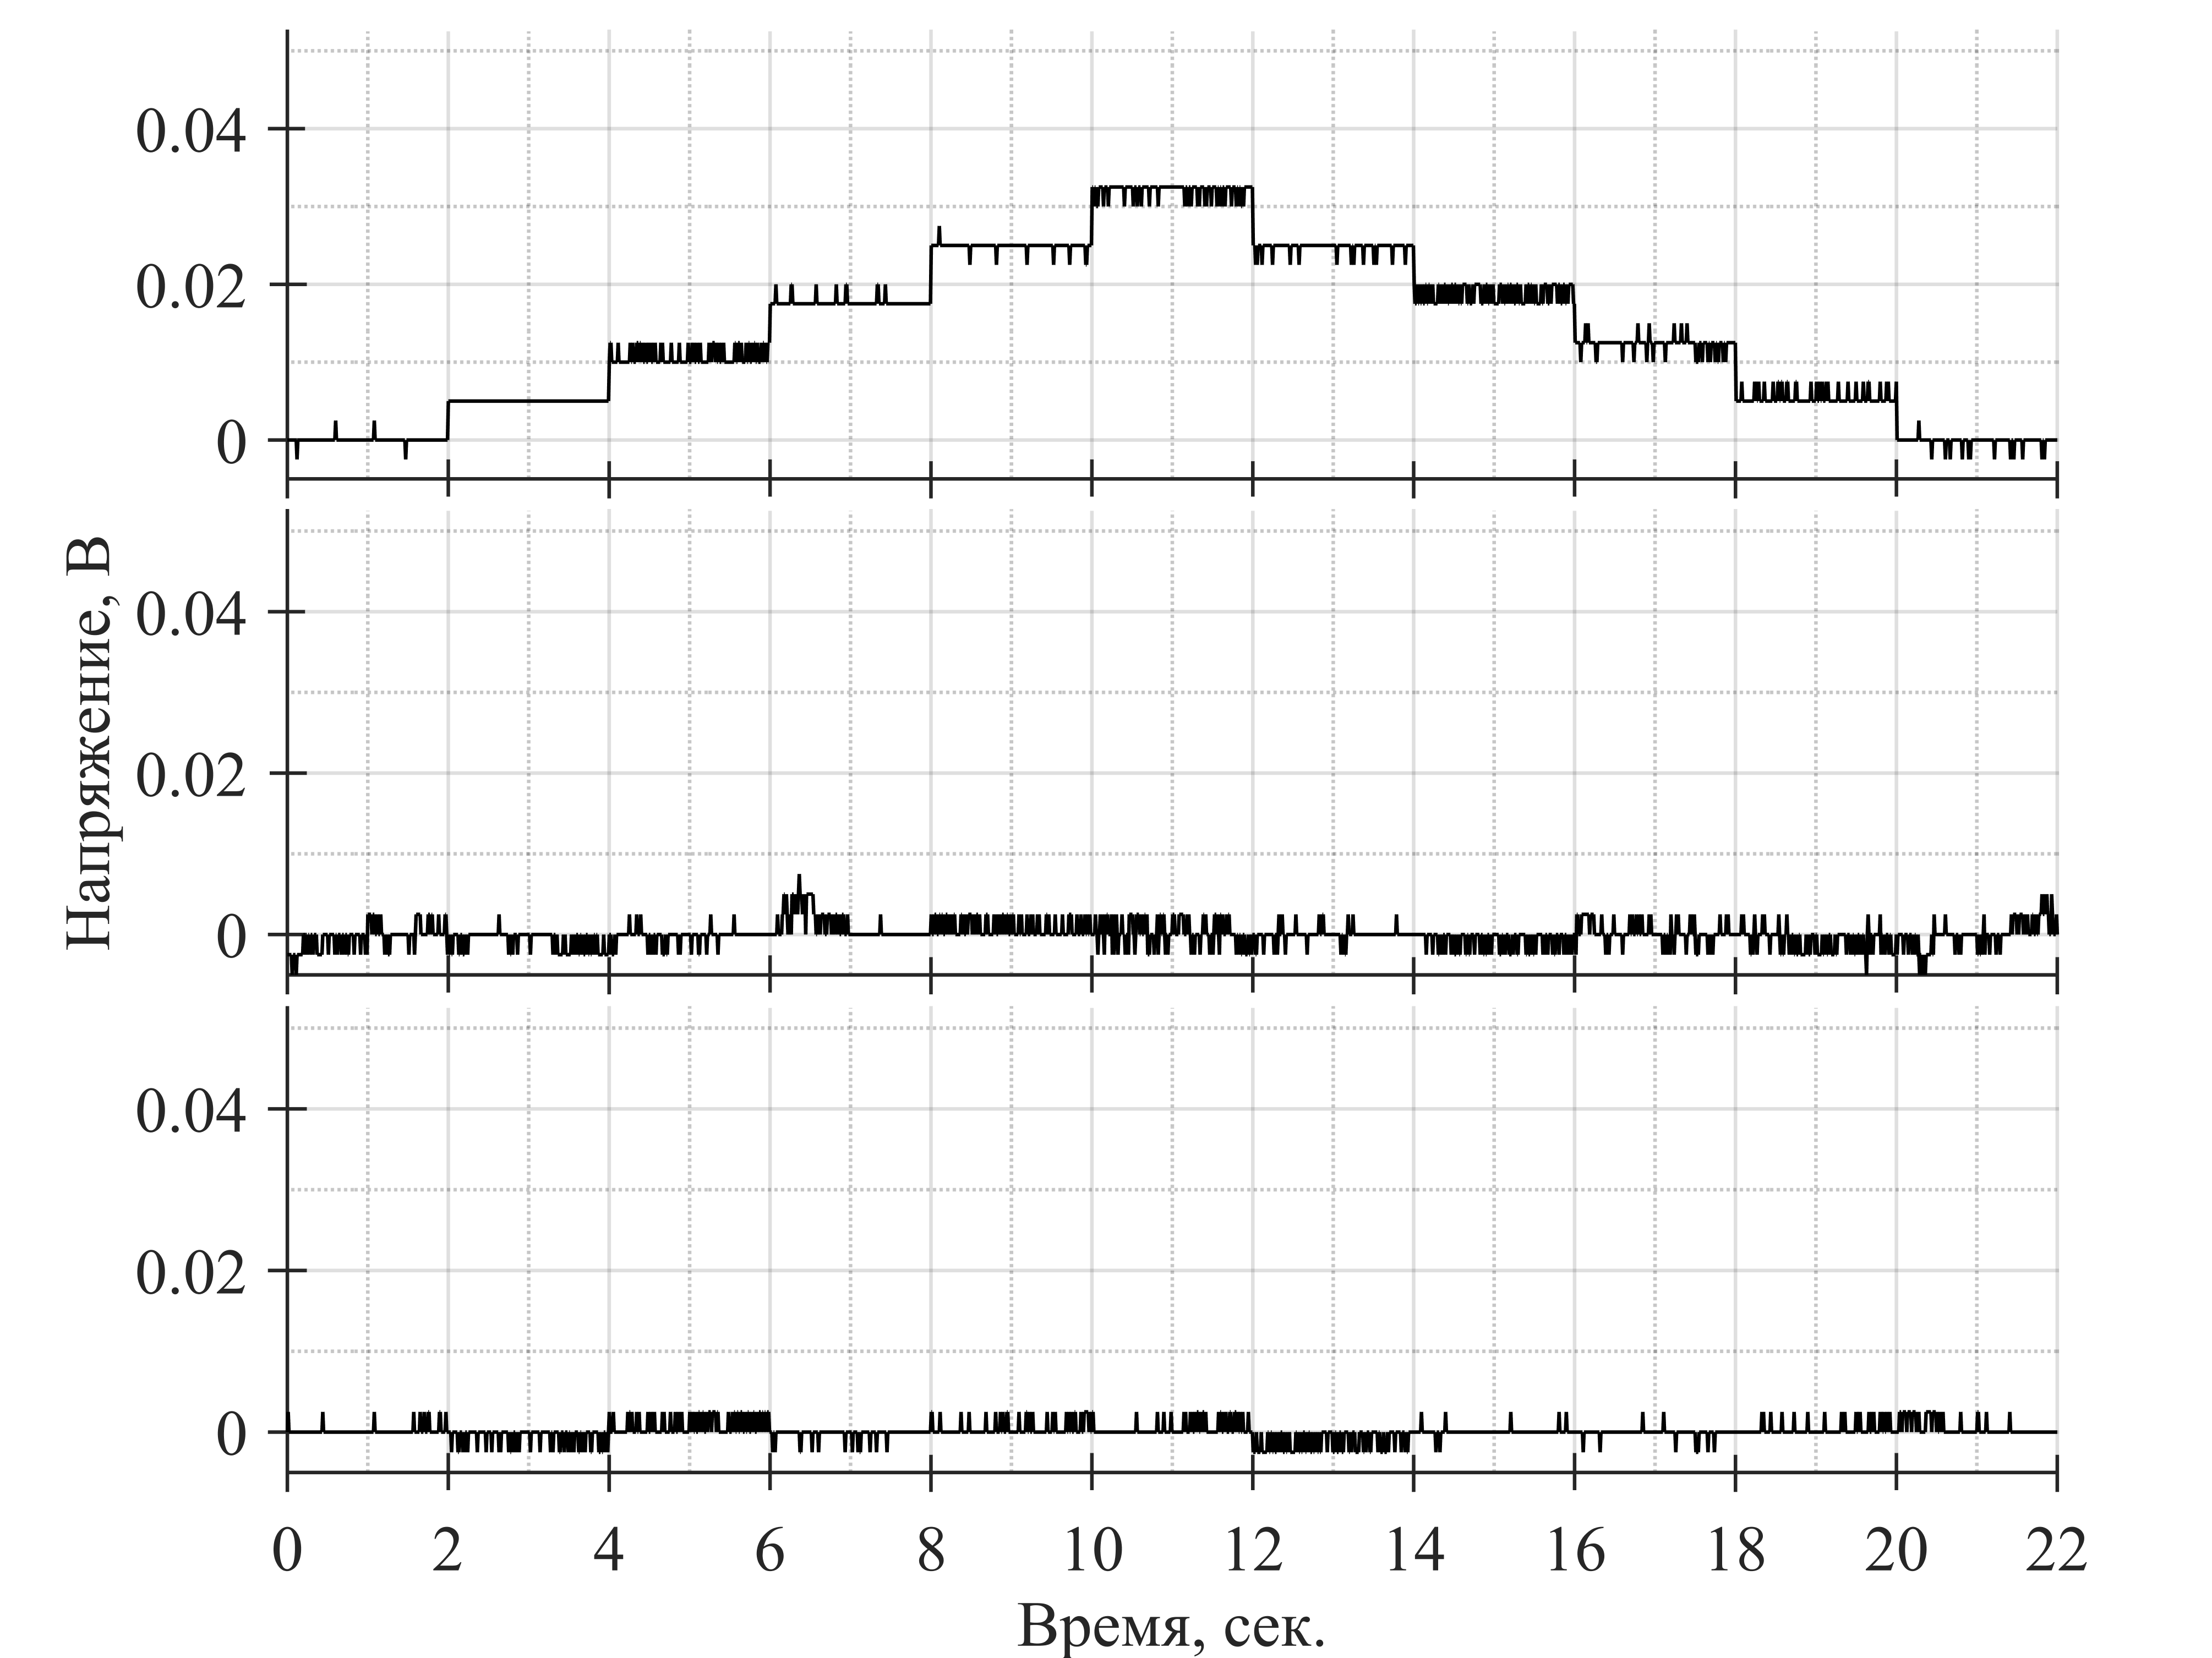
\includegraphics[width=0.86\textwidth]{CalibrationRawHor}
	
	С веху вниз: горизонтальная, боковая, вертикальная составляющие усилия резания
	\caption{Диаграмма переходных процессов при тарировании горизонтальной составляющей усилия резания}  
	\label{fig:CalibrationRawHor}  
\end{figure}
Используя данные из диаграммы приведенной на рисунке~\ref{fig:CalibrationRawHor} составим таблицу~\ref{tab:DCHor} зависимости напряжения, снимаемого с тензометрических датчиков, от прилагаемого, к тензометрическому звену, усилия.
\begin{table}[htp]
	\centering
	\caption{Зависимость напряжения на каналах оцифровки от приложенной силы в процессе тарирования горизонтальной составляющей усиля резания}
	\label{tab:DCHor}
	\begin{tabular}{|r@{ }l|r@{,}l|r@{,}l|r@{,}l|}
		\hline
		\multicolumn{2}{|c|}{\multirow{2}{*}{Сила, Н}} & \multicolumn{6}{c|}{Канал измерения} \tabularnewline
		\cline{3-8}
		\multicolumn{2}{|c|}{}   & \multicolumn{2}{c|}{горизонтальный, мВ}  & \multicolumn{2}{c|}{боковой, мВ} & \multicolumn{2}{c|}{вертикальный, мВ}\tabularnewline
		\hline
		\hline
		&0                          & 0&0687                                               & 0&175         & 0&325\tabularnewline
		&500                        & 5&19                                                 & 0&769         & 0&406\tabularnewline
		1&000                       & 11&5                                                 & 0&212         & 0&456\tabularnewline
		1&500                       & 18&2                                                 & 0&919         & 0&106\tabularnewline
		2&000                       & 24&9                                                 & 0&438         & 0&787\tabularnewline
		2&500                       & 32&1                                                 & 0&25          & 0&412\tabularnewline
		\hline
	\end{tabular}
\end{table}

\pagebreak

Используя табличные данные (см. таблицу~\ref{tab:DCHor}) можно получить зависимости изображенные на рисунке~\ref{fig:Calibration}. Из них видно что силы возникающие на тензометрическом звене имеют линейную зависимость от напряжения получаемого с тензометрических мостов. 
\begin{figure} [!ht]
	\centering
	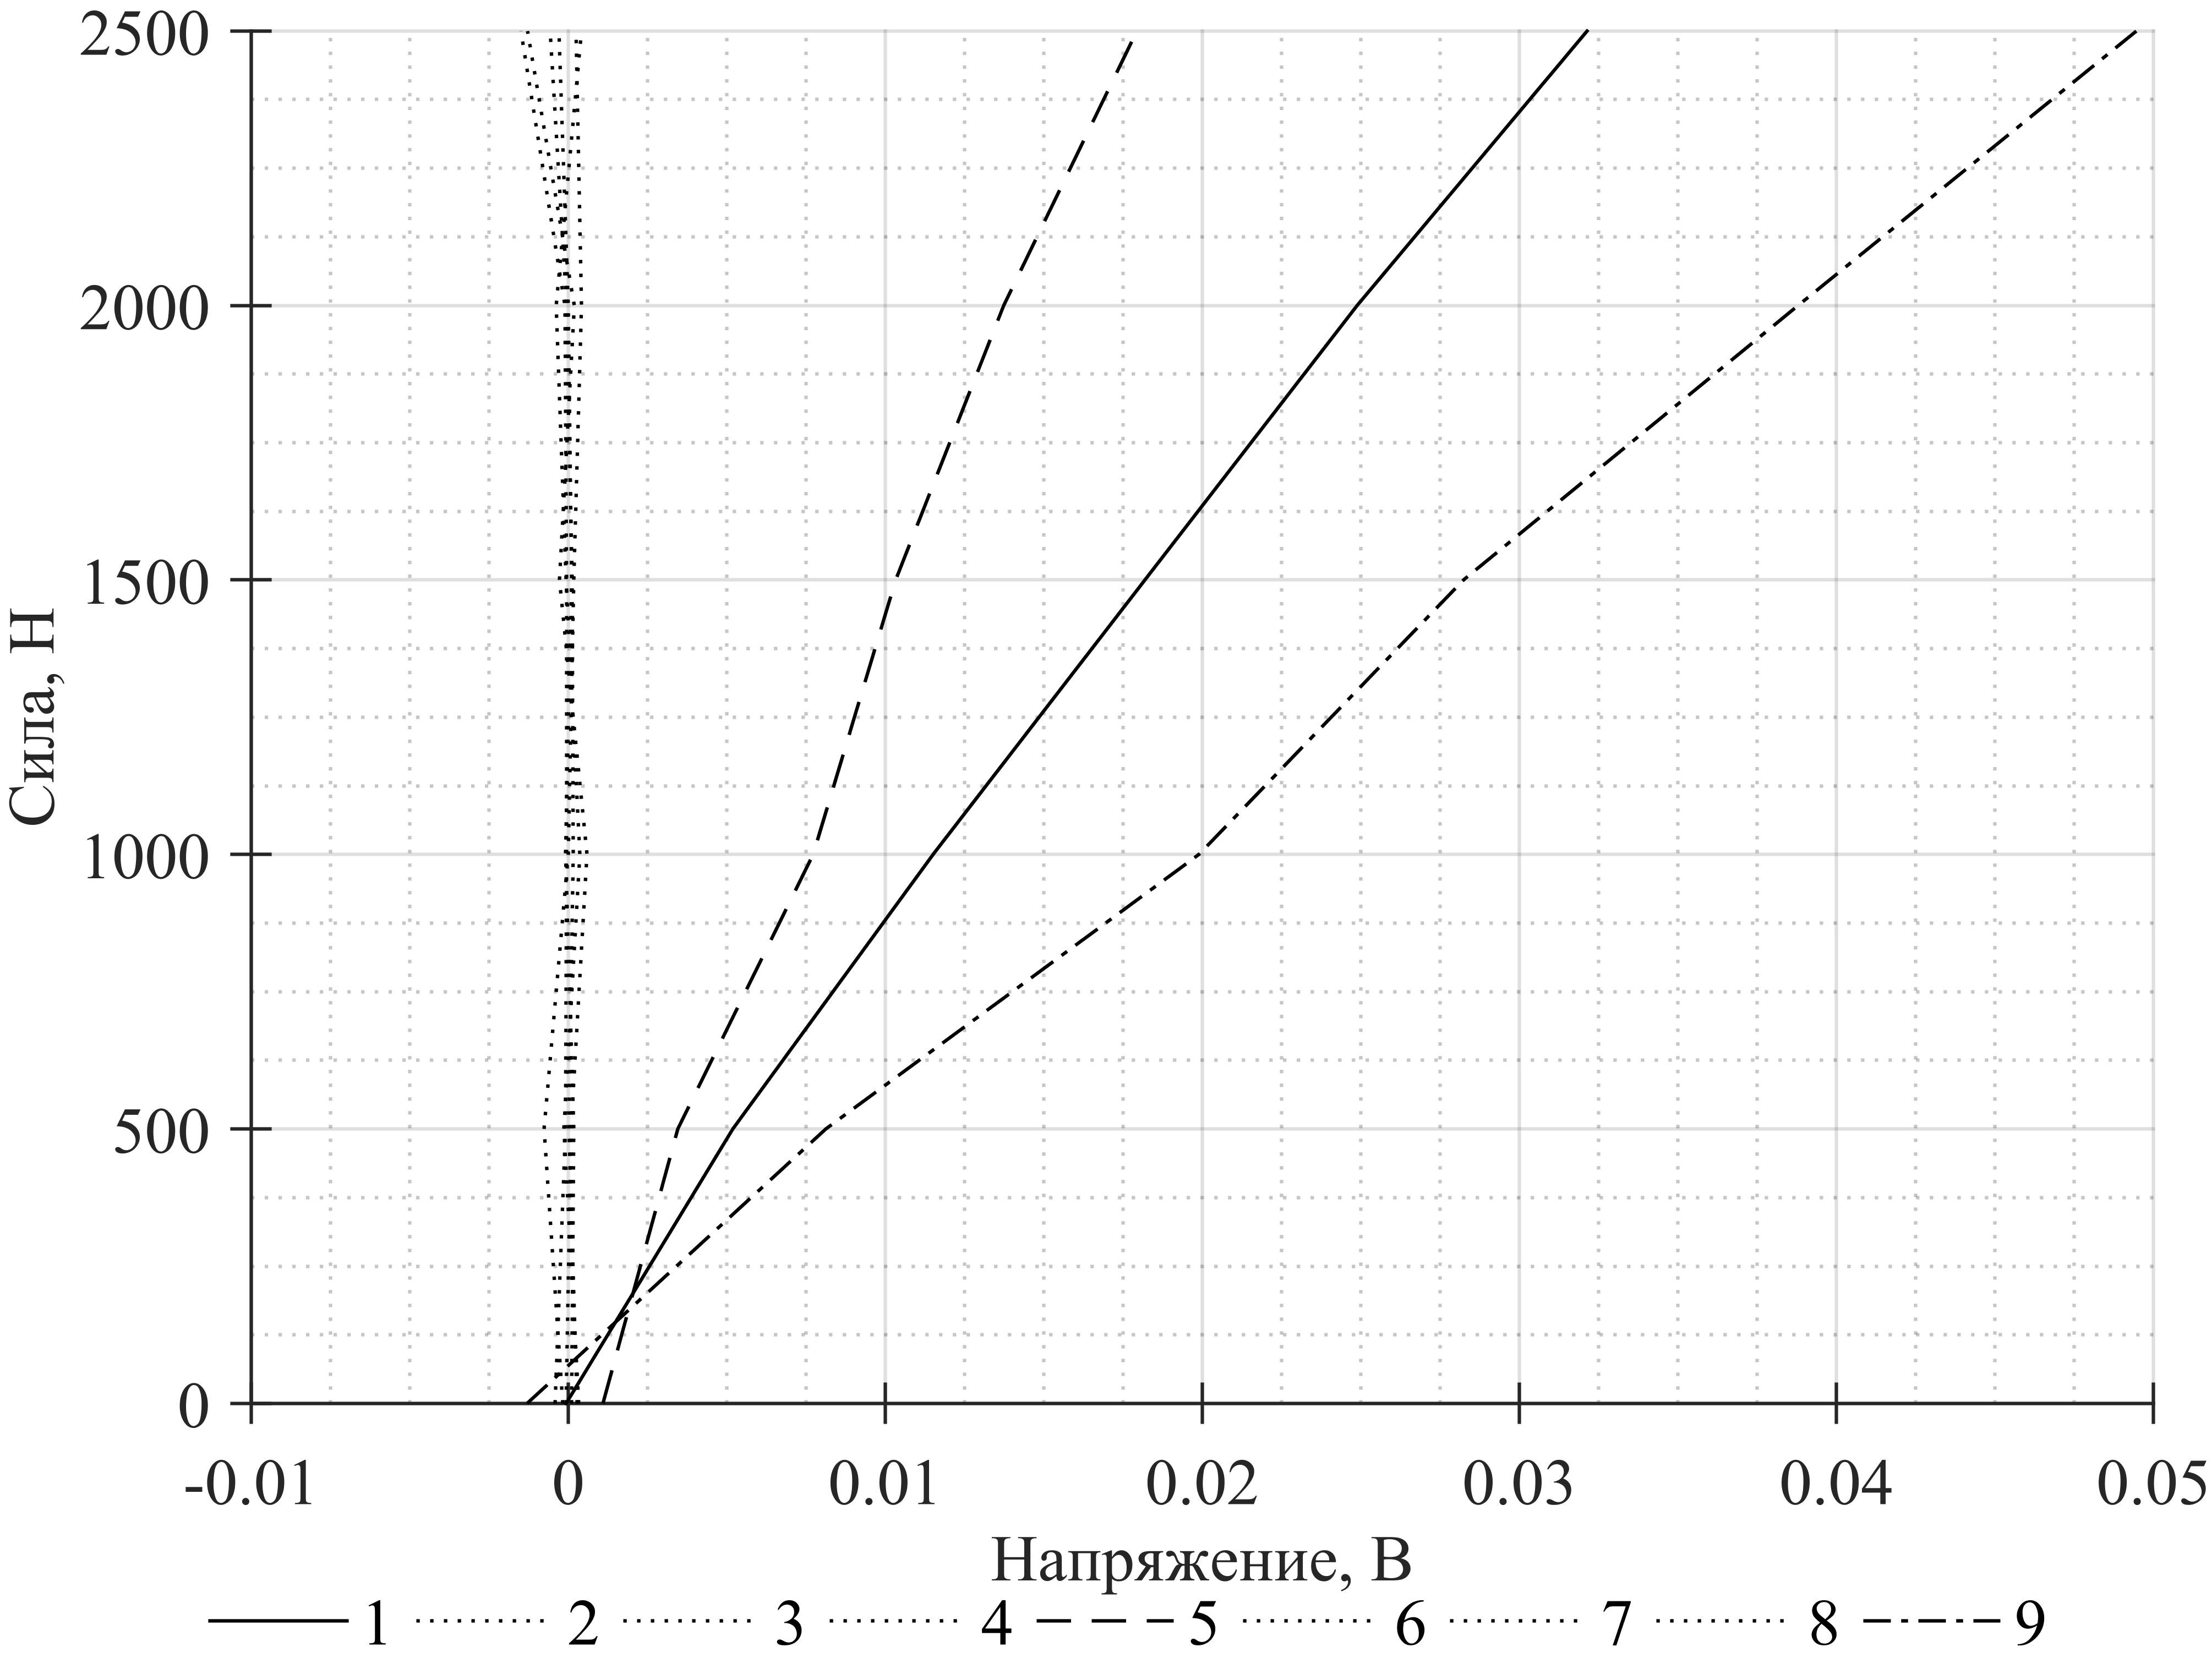
\includegraphics[width=0.85\textwidth]{Calibration.png}
	
	1, 2, 3 "--- горизонтальная, бокова, вертикальная составляющие усилия резания соответственно при тарировании горизонтальной составляющей; 4, 5, 6 "--- аналогично  при тарировании боковой составляющей; 7, 8, 9 "--- аналогично при тарировании вертикальной составляющей.
	\caption{Графики тарирования тензометрического звена}
	\label{fig:Calibration}  
\end{figure}

% Эти графики можно представить в виде уравнений:
% \begin{alignat}{2}
% 	y_\text{гор}  & = 80~&074,568 \cdot x  \label{eq:TrendHor}\\
% 	y_\text{бок}  & = 140~&953,396 \cdot x \label{eq:TrendLat}\\
% 	y_\text{верт} & = 51~&338,284 \cdot x \label{eq:TrendVert}
% \end{alignat}
Из 
%уравнений \labelcref{eq:TrendHor,eq:TrendLat,eq:TrendVert} 
таблицы~\ref{tab:DCHor}
получим тарировочные коэффициенты: 8~0074,568~$ \slantfrac{\text{Н}}{\text{В}} $, 140~953,396~$ \slantfrac{\text{Н}}{\text{В}} $, 51~338,284~$ \slantfrac{\text{Н}}{\text{В}} $ для горизонтальной, боковой и вертикальной составляющей усилия резания соответственно.

\section{Выводы}

Тарирование измерительного преобразователя является одним из важнейших факторов успешности проведения экспериментальных исследований. Известно, что на его показания может оказывать влияние множество различных переменных, например: электро магнитные поля; сопротивление проводов; температура окружающей среды. Выявление таких влияний на этапе тарирования, позволяет или полностью их устранить или заложить их учет в тарировочный коэффициент, что в свою очередь сказывается на данных полученных в ходе экспериментальных исследований. Тарирование следует проводить перед каждой серией экспериментов. Также перед каждым тарированием рекомендуется проводить тренировку измерительного преобразователя, загрузка разгрузка несколько раз, без фиксации получаемых данных. Это позволяет \todo{...}.

Корректность и аккуратность тарирования влияет на точность будущих измерений, так как все измерения будут домножены на тарировочный коэффициент. Также в процессе тарирования измерительного преобразователя могут быть выявленны сбои в его работе, поломки. Что позволит своевременно их устранить и обеспечить целостность экспериментальных данных.